%% josis.tex 1.4   2016-09-15    JoSIS latex template
%------------------------------------------------------------------
% Filename: josis_template.tex
%
% This file is intended as a template for typesetting articles for the
%
%                        Journal of Spatial Information Science.
%
% Please edit this template to generate your own formatted manuscripts
% for submission to JOSIS. See http://josis.org for further details.
%


%%% JOSIS checks in typesetting
%%% * All titles and sections lower case *EXCEPT short title  [ ]
%%% * Remove author postal addresses, only have geographic places and institutions [ ] 
%%% * Consistent use of Section, Figure, Table (capitalized and in full) [ ]
%%% * 10 keywords (and all lower case) [ ]
%%% * Remove all avoidable footnotes [ ]
%%% * Use double quotation marks (``'' not "" or `') [ ]
%%% * Punctuation inside quotations [ ]
%%% * E.g. and i.e. followed by comma [ ]
%%% * cf. followed by tilde [ ]
%%% * Itemize and enumerate correctly punctuated [e.g., "1. x, 2. y, and 3. x." ]
%%% * And/or lists using American English punctuation (e.g., "x, y, and z") [ ] 
%%% * Bibliography (e.g., en-dashes for number ranges, consistent "Proc.~" for Proceedings of..., etc.) []
%%% * Acknowledgment style use section* [ ] 
%%% * et al. no italics, but with dot  [ ] 
%%% * All captions end with full stop  [ ] 
%%% * Table captions under, not over table  [ ]
%%% * Adjust urls with burlalt [ ] 
%%% * Check correct use of hyphens, emdashes, endashes  [ ]
%%% * Perform spell check  [ ] 

%%% JOSIS checks directly before publication 
%%% Check DOI, page numbers on article and web site. [ ]
%%% Update web site with final title, abstract, keywords. [ ] 
%%% Build with distiller for DOI links. [ ]


% Required documentclass definition for JOSIS
\documentclass{josis}
\usepackage{hyperref}
\usepackage[hyphenbreaks]{breakurl}
\usepackage{booktabs}
\usepackage{stmaryrd}
\usepackage[T1]{fontenc}
\usepackage{cite}
\usepackage{subcaption}
% Suggested packages for algorithm formatting
\usepackage{algorithm}
%\usepackage{algorithmic}
\usepackage{algpseudocode}
\usepackage{pythonhighlight}
%\usepackage{natbib}
\usepackage{amssymb,amsmath}
%\usepackage[table]{xcolor}
\usepackage{lastpage}
\renewcommand{\topfraction}{0.9} 
\renewcommand{\textfraction}{0.1}
% Page setup and overhangs
\sloppy
\widowpenalty=10000
\clubpenalty=10000
\hyphenpenalty=75
% Article details for accepted manuscripts will be added by editorial staff
% Omit year if article in press
% Omit number if article under review
\josisdetails{%
   number=2, year=2024, firstpage=1, lastpage=\pageref{LastPage}, 
  doi={IUCP-2024},
  % received={December 24, 2015}, 
   %returned={February 25, 2016},
   %revised={July 13, 2016},
   %accepted={September 5, 2016},
   }

%\newcommand{\mydoi}[1]{\href{http://dx.doi.org/#1}{doi:\protect\detokenize{#1}}}

%\renewcommand{\UrlLeft}{http:\sslash}
%\DeclareUrlCommand\myurl{\def\UrlLeft{}\def\UrlRight{}%
%\urlstyle{tt}}

\urlstyle{rm}
\makeatletter
% Inspired by http://anti.teamidiot.de/nei/2009/09/latex_url_slash_spacingkerning/
% but slightly less kern and shorter underscore
\let\UrlSpecialsOld\UrlSpecials
\def\UrlSpecials{\UrlSpecialsOld\do\/{\Url@slash}\do\_{\Url@underscore}}%
\def\Url@slash{\@ifnextchar/{\kern-.11em\mathchar47\kern-.2em}%
    {\kern-.0em\mathchar47\kern-.08em\penalty\UrlBigBreakPenalty}}
\def\Url@underscore{\nfss@text{\leavevmode \kern.06em\vbox{\hrule\@width.3em}}}
\makeatother

\hypersetup{
colorlinks=true,
linkcolor=black,
citecolor=black,
urlcolor=black
} 

% Add the running author and running title information
\runningauthor{\begin{minipage}{.9\textwidth}\centering Anjana Vinod, Leya Kurian , Lisbeth Ajith \end{minipage}}
\runningtitle{Restaurant Revenue Prediction}

% Document begins
\begin{document}
%\setcounter{page}{33}


% Insert your own title
\title{Restaurant Revenue Prediction Using Machine Learning}

% Insert your manuscipts authors, affiliations, and addresses
\author{Anjana Vinod}
\author{Leya Kurian }
\author{Lisbeth Ajith}\affil{Saintgits Group of Institutions, Kottayam, Kerala}
\date{}
\maketitle
% Add 5-10 keywords for every submission
\keywords{Machine Learning,prediction,Customer reviews, Restaurant revenue Linear regression,SVM,Decision trees,KNN,XGB regressor,LightGBM,Supervised models,Unsupervised models}
% Add a short abstract of 150-250 words 
\begin{abstract}
This project focuses on predicting restaurant revenue using a dataset of 1000 samples, leveraging diverse input features such as customer metrics, menu prices, marketing expenditures, and promotion activities. Initial explorations with supervised regression models such as Linear Regression, SVM, and Decision Trees yielded suboptimal results. Transitioning to classification algorithms—Logistic Regression, SVM, K-Means, Decision Trees, and Random Forests—improved predictive accuracy. Unsupervised techniques were also employed to validate classification findings. The study emphasizes the importance of utilizing various machine learning methodologies iteratively. By combining regression, classification, and clustering approaches, enhanced revenue prediction accuracy was achieved, providing valuable insights for informed decision-making in the restaurant industry \cite{ismail2023predicting}. This holistic approach underscores the significance of comprehensive model selection and iterative refinement to effectively address real-world prediction challenges.
\end{abstract}
% Your main text begins here. 
\section{Introduction}
This project investigates restaurant revenue prediction using both supervised and unsupervised classes of machine learning algorithms. The project aims to improve revenue forecasting within the restaurant industry by exploring a dataset of 1,000 samples that includes diverse input features such as customer metrics, menu prices, marketing expenses, and promotional activities. Through an examination of supervised regression models and classification algorithms, along with unsupervised clustering techniques, the study seeks to enhance prediction accuracy and provide actionable insights for decision-making processes in restaurant management. By analyzing these algorithmic approaches, the research aims to contribute standardized methodologies for effective revenue prediction, thereby supporting informed decision-making practices within the restaurant sector.
\section{Libraries Used}
In the project for various tasks, following packages are used.
\begin{python}
Pandas
Matplotlib
Seaborn
Scikit-learn
LightGBM (lgb)
XGBoost (xgb)
\end{python}
\section{Literature Review}
The researchers Md Yasin Ali Parh, Mst Sharmin Akter Sumy, and Most Sifat Muntaha Soni 
\cite{redy2021restaurant,redy2023restaurant,ismail2023predicting,shah2016restaurant} applied multiple machine learning models, including linear regression, ridge regression, random forest, and gradient boosting, to predict restaurant revenue.Among these models, ridge regression demonstrated the highest accuracy, achieving a mean squared error of 3.46.

In the study titled "Restaurant Revenue Prediction Applying Supervised
Learning Methods" conducted by Md Yasin Ali Parh, Mst Sharmin Akter Sumy, and Most Sifat Muntaha Soni \cite{ismail2023predicting}, the LASSO method displayed the highest accuracy with a mean squared error of approximately 2.7. This approach was used as the machine learning model for predicting restaurant revenue.
\section{Methodology}
In this work, two types of models are used. For the first part, various Regression models are used but the $R^2$ values produced range between 0.2 to 0.64 which is not sufficient. Hence we tried for classification models.
The linear regression model is represented as:
\begin{equation}
         \hat{\mathbf{y}} = \mathbf{X}\beta + \epsilon
\end{equation}
where $\hat{\mathbf{y}}$ is the predicted restaurant revenue, $\beta$ is the vector of coefficients, and $\epsilon$ is the error term.

The objective of linear regression is to minimize the sum of squared errors (SSE), given by:
\begin{equation*}
    SSE = \sum_{i=1}^{n} (y_i - \hat{y}_i)^2
\end{equation*}
where $y_i$ is the actual revenue and $\hat{y}_i$ is the predicted revenue for sample $i$. This is achieved by estimating the coefficients $\beta$ using the least squares method:
\begin{equation*}
    \hat{\beta} = (\mathbf{X}^T\mathbf{X})^{-1}\mathbf{X}^T\mathbf{y}
\end{equation*}
\subsubsection*{Support Vector Machine Regression}
\[
f(x) = \sum_{i=1}^{n} \alpha_i y_i K(x_i, x) + b
\]

SVM Regression predicts the output based on a weighted sum of support vectors' target values with kernel transformations, adjusted by Lagrange multipliers and a bias term.

\subsubsection*{Decision Trees Regression}
Decision trees recursively split the feature space based on feature thresholds to minimize the variance of the target variable within each node, leading to piecewise constant predictions.

\subsubsection*{K-Nearest Neighbors (KNN) Regression}
The objective in kNN is implicit in the choice of distance metric and $k$ value, aiming to find the optimal combination that minimizes the chosen error metric,
\[
f(x) = \frac{1}{k} \sum_{i=1}^{k} \left(y_i-f(x_i)\right)^2
\]

KNN Regression predicts the output as the average of the target values of the \( k \) nearest neighbors of the input sample \( x \).

Some of the classification algorithms used in this project are given below.
\subsubsection*{Logistic Regression}
\begin{equation*}
        \[p(y=1 \,|\, x) = \frac{1}{1 + e^{-(b + \sum_{i=1}^{n} w_i x_i)}}\]
\end{equation*}\]
Logistic Regression models the probability of the target variable belonging to class 1 given the input features using a sigmoid function, with weights \( w_i \) and a bias term \( b \).
\subsubsection*{Support Vector Machine (SVM) Classifier}

SVM Classifier predicts the class label based on the sign of the decision function, which is a weighted sum of support vectors target values with kernel transformations, adjusted by Lagrange multipliers and a bias term.
\[
f(x) = \sum\limits_{i=1}^{n} \alpha_i y_i K(x_i, x) + b
\]

\section{Implementation}
In the initial step of the methodology, comprehensive data preprocessing was carried out to ensure the quality and integrity of the dataset. This process included multiple stages, such as data cleaning, removal of negative values, and handling missing values. No missing data were identified within the features, and categorical variables were encoded using one-hot encoding to facilitate model training. Additionally, feature scaling was performed using StandardScaler to standardize the numerical features, bringing them to a uniform scale and preventing any single feature from dominating the model training process. Below are some illustrations of cuisine type and outlier detection.

\begin{figure}[t]
    \centering
    \begin{subfigure}[b]{0.65\textwidth}
        \centering
        \caption{Cuisine Type}
        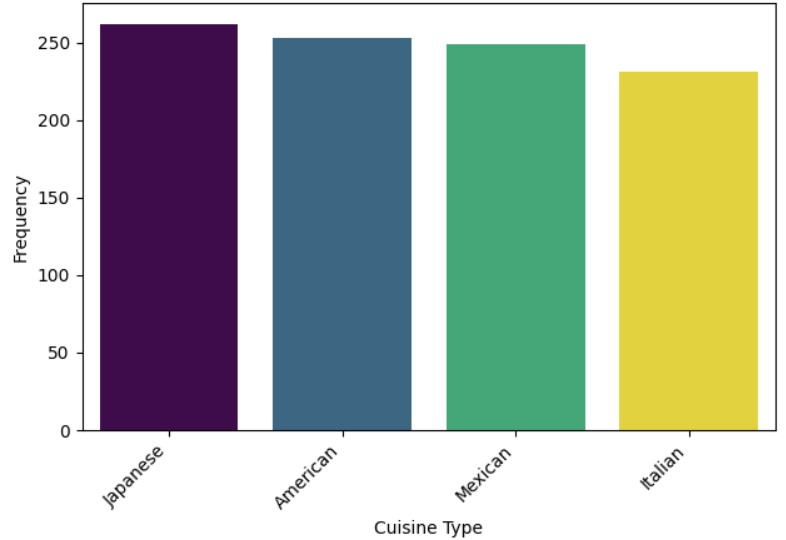
\includegraphics[width=\textwidth]{cuisinetype.jpg}
        \label{fig:subfig1}
    \end{subfigure}
    \centering
    \begin{subfigure}[b]{0.95\textwidth}
        \centering
        \caption{Outlier Detection}
        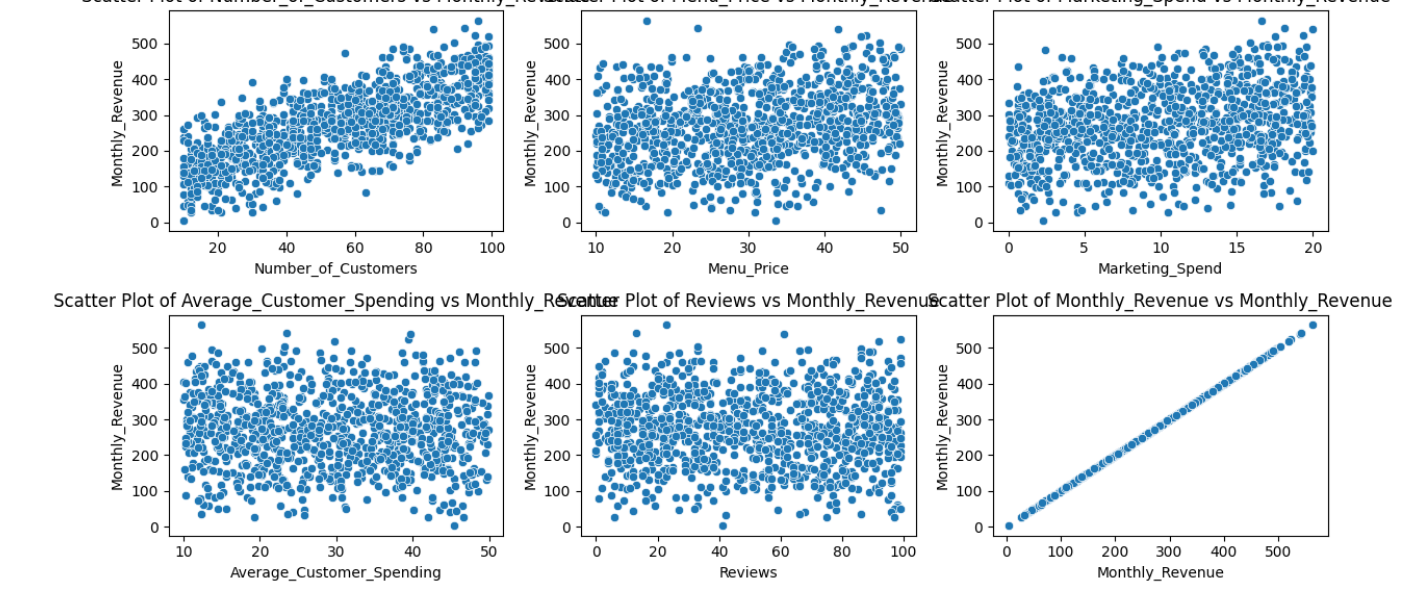
\includegraphics[width=\textwidth]{outlier.png}
        \label{fig:subfig2}
    \end{subfigure}
    \hfill
\end{figure}


After preprocessing the data, the next step was to select suitable machine learning algorithms for the revenue prediction task. Given the nature of the problem as a regression task, regression algorithms such as Random Forest Regressor, Gradient Boosting Regressor, and Support Vector Regressor were chosen. These algorithms were selected based on their ability to capture complex nonlinear relationships within the data and their proven performance in similar prediction tasks. The scikit-learn library was used to implement these algorithms, and their hyperparameters were fine-tuned using techniques such as grid search and cross-validation to optimize performance.

After conducting extensive experimentation with regression models, including Random Forest Regressor and Gradient Boosting Regressor, the models exhibited limited success in accurately predicting restaurant revenue. This limited success may be attributed to the complex and nonlinear nature of the data. Consequently, the focus shifted to exploring classification models to effectively categorize revenue levels. The aim was to gain deeper insights into revenue patterns and enhance predictive performance.A total of seven different regression algorithms were tested (four classical and three ensemble methods). The accuracy of these models ranged from 0.2 to 0.64. Additionally, exploratory data analysis (EDA) revealed no significant linear association between input and target variables. Given these observations, classification models were considered as an alternative approach.

The initial step in the methodology entailed comprehensive data preprocessing to ensure the quality and integrity of the dataset. This process comprised various stages, including data cleaning, eliminating negative values, and handling missing values. No missing data were found within the features, and categorical variables were encoded using one-hot encoding to facilitate model training. Additionally, feature scaling was carried out using the StandardScaler to standardize the numerical features and bring them to a uniform scale, thus preventing any particular feature from dominating the model training process. Below are some illustrations depicting cuisine type, outlier detection, and examining dependency between the features.

The results of these implementations are discussed in the next section.
\section{Results \& Discussion}
 A summary of the results is shown in Table
 \ref{tab:large-model}.
\begin{table}%[htp]
\centering
\caption{Summary of regressor models tested for prediction }
\label{tab:large-model}
\begin{tabular}{|c|l|c|c|c|c|c|l|}
\hline
\begin{tabular}[c]{@{}c@{}}Model\\ No.\end{tabular} & \multicolumn{1}{c|}{Model Name} & \begin{tabular}[c]{@{}c@{}}MSE\\\end{tabular} & RMSE & Rsquared value & \multicolumn{1}{c|}{\begin{tabular}[c]{@{}c@{}}Processing\\ Time\end{tabular}} \\ \hline
1. & Linear Regression & 3583.8920 & 59.8656 & 0.6492 & 50.6799 sec \\ \hline
2. & Decision Tree & 6514.7520 & 80.7140 & 0.3623 & 121.9058 sec \\ \hline
3. & SVM & 8638.5058 &  92.9435 & 0.2091 & 1.0051 sec  \\ \hline
4. &Random forest&  4033.0267 & 63.5061 & 0.6307 & 0.0232 sec \\ \hline
5.& XGB regressor    &4784.1573 &69.1676 &0.5620 &0.0034 sec \\ \hline
6.& LightGBM    &3939.5446 &62.7657 &0.6393 &0.0036 sec \\ \hline
7.& KNN    &4621.7702 &67.98360 &0.5769 &0.8590 sec \\ \hline
\end{tabular}
\end{table}

 Seven different regression algorithms were evaluated, including four classical models and three ensemble models. The $R^2$ values ranged from 0.2 to 0.64. Exploratory data analysis (EDA) revealed no significant linear association between input and target variables. As a result, classification models were explored as an alternative approach. The results of this analysis are presented in Table \ref{tab:intel_model}.

\begin{table}%[htp]
\caption{Summary of classification models tested}
\label{tab:intel_model}
\begin{tabular}{|c|l|c|c|c|c|c|l|}
\hline
\begin{tabular}[c]{@{}c@{}}Model\\ No.\end{tabular} & \multicolumn{1}{c|}{Model Name} & \begin{tabular}[c]{@{}c@{}}Accuracy\\ \end{tabular} & precision & f1-score & Recall & \multicolumn{1}{c|}{\begin{tabular}[c]{@{}c@{}}Processing\\ Time\end{tabular}} \\ \hline
1. & Logitsic Regression & 0.6834 & 0.6724 & 0.6834 & 0.6767 & 0.0097 sec \\ \hline
2. & Decision Tree & 0.6080 & 0.6226 & 0.6080 & 0.6143 & 1.4707 sec \\ \hline
3. & Random forest classifier & 0.6633 & 0.6566 & 0.6633 & 0.6592 &  0.0127  sec \\ \hline
4.& SVM Classifier &0.6582 &0.6615 &0.6582 &0.6598 &0.0123 sec\\ \hline
5.& Naive Bayes classifier & 0.6633 &0.6531 &0.6633 &0.6496 & 0.0480 sec\\ \hline
6.& KNN Classifier &0.6381 &0.6501 &0.6381 &0.6407 &0.0142 sec\\ \hline
\end{tabular}
\end{table}
K-means clustering was utilized as part of the classification models. It achieved an accuracy of 0.44; however, its performance was lower compared to other classification methods tested. This relatively low accuracy suggests that K-means may not be the most suitable approach for predicting restaurant revenue in this dataset. Nonetheless, the clustering method still provided some insights, though other models such as logistic regression and decision trees outperformed it significantly.
\section{Conclusions}
This project focused on optimizing restaurant revenue prediction by utilizing various input features and machine learning methodologies. While initial regression models showed limited performance, subsequent classification algorithms demonstrated improved accuracy, with unsupervised clustering methods supporting the findings. The approach was characterized by a diverse selection of methods and iterative refinement, yielding valuable insights for informed decision-making in the restaurant industry. The study highlights the significance of iterative adaptation of machine learning techniques to address real-world prediction challenges, thereby enhancing revenue prediction accuracy and supporting strategic decision-making within the restaurant sector.
\section*{Acknowledgments}
We extend our sincere gratitude to Intel for their support and contributions to this restaurant revenue prediction project. Their cutting-edge technology and resources have been instrumental in enabling us to explore innovative approaches and achieve meaningful insights. We also acknowledge the invaluable assistance and collaboration of our team members, whose dedication and expertise have been indispensable throughout this endeavor. Additionally, we express our appreciation to the restaurant industry stakeholders and dataset providers for their valuable contributions. This project would not have been possible without the collective efforts and support of all involved parties. 

Furthermore, we would like to extend special acknowledgment to Prof.~Siju Swamy for his exceptional mentorship. His guidance and insights have been pivotal in shaping the direction of this project and fostering our growth as individuals and as a team. We are truly grateful for his mentorship and unwavering support throughout this journey.

\bibliographystyle{josisacm}
\bibliography{josisexample}
% \cite{redy2021restaurant, redy2023restaurant, ismail2023predicting, shah2016restaurant}
\section{Main code sections for the solution}
\subsection{Loading data from the source}
Data for this project is taken from kaggle: \url{https://www.kaggle.com/datasets/mrsimple07/restaurants-revenue-prediction}. The python code section for this stage is shown bellow:
\begin{python}
csv_file_path = 'restuarant_revenueDB.csv'
res = pd.read_csv(csv_file_path)
\end{python}
\subsection{Python function for visualization}
The general function for basic EDA of the data is created in python. The code for this task is given bellow:
\begin{python}
numeric_data = res1.select_dtypes(include='number')

# Compute correlation matrix
correlation_matrix = numeric_data.corr()

# Plot heatmap
plt.figure(figsize=(10, 8))
sns.heatmap(correlation_matrix, annot=True)
plt.show()

\end{python}
\subsection{Data cleaning \& pre-processing}
Python code for checking for missing values, creation of meaning ful news content from the data and other preprocessing task are shown bellow:
\begin{python}
# to remove negative values inside a column
import pandas as pd
res = res[res['Monthly_Revenue'] >= 0]
res.isnull().sum()
res.duplicated().sum()
print(res)
\end{python}   
\begin{python}
# split data into features(X) and target variable(y) in regression models
X = res.drop(['Monthly_Revenue'], axis =1)
y = res['Monthly_Revenue']
# split data into features(X) and target variable(y) in classification  models
X = res1.drop(['Revenue_category','Cuisine_Type'], axis =1)
y = res1['Revenue_category']

#Data preprocessing
from sklearn.preprocessing import StandardScaler

# Initialize the StandardScaler
scaler = StandardScaler()

# Fit the scaler to your data and transform it
X_scaled = scaler.fit_transform(X)

\end{python}
\subsection{Dataset preperation}
Splitting the dataset into training and testing sets.It helps to avoid overfitting and to accurately evaluate your model.  
\begin{python}
#split the data into training and testing sets
X_train, X_test, y_train, y_test=train_test_split(X,y,test_size=0.2,
random_state=42)
\end{python}
\subsection{Model Training\& Evaluation}
Model training is done on the basis of machine learning algorithms such as Naive Bayes,Logistic Regression or Decision tree using the training set and extracted features.The model is then evaluated using metrics such as accuracy, precision, recall, and F1-score.
\begin{python}
#linear regression
model = LinearRegression()
model.fit(X_train, y_train)
y_pred = model.predict(X_test)
 
#Decision tree regressor
regressor = DecisionTreeRegressor(random_state=42)
# Train the regressor on the training set
regressor.fit(X_train, y_train)
# Make predictions on the test set
y_pred = regressor.predict(X_test)
 
#SVM regressor
# Train the Support Vector Regression (SVR) model
svr_model = SVR(kernel='rbf')  # Using radial basis function kernel
svr_model.fit(X_train_scaled, y_train)
y_pred = svr_model.predict(X_test_scaled)


#Random Forest regression
rf_model = RandomForestRegressor(n_estimators=100, random_state=42)  # Using 100 trees
rf_model.fit(X_train_encoded, y_train)
y_pred = rf_model.predict(X_test_encoded)

#XGB Regressor
xgb_model = XGBRegressor(n_estimators=100, random_state=42)  # Using 100 trees
xgb_model.fit(X_train, y_train)
y_pred = xgb_model.predict(X_test)

#LightGBM
lgb_train = lgb.Dataset(X_train, y_train)
lgb_eval = lgb.Dataset(X_test, y_test, reference=lgb_train)
gbm = lgb.train(params,
                lgb_train,
                num_boost_round=100,
                valid_sets=[lgb_train, lgb_eval])  # Print evaluation
y_pred = gbm.predict(X_test, num_iteration=gbm.best_iteration)

#KNN
knn_model = KNeighborsRegressor(n_neighbors=5)  # Initialize KNN model with 5 neighbors
knn_model.fit(X_train, y_train)
y_pred = knn_model.predict(X_test)
\end{python}
Performed 7 different regression algorithms(4 classical,3 ensemble).The $R^2$
 -values range from 0.2 to 0.64.Also from EDA there is no significant linear association between input and targer variables is observed.So we will try classification models.
 \begin{python}
 #Logistic Regression
 model = LogisticRegression()
 model.fit(X_train, y_train)
 y_pred = model.predict(X_test)

#Decision Tree
clf = DecisionTreeClassifier(criterion="entropy")
clf.fit(X_train, y_train)
y_pred = clf.predict(X_test)

#K means clustering
k = 3 # Number of clusters
kmeans = KMeans(n_clusters=k,n_init='auto', random_state=42)
kmeans.fit(X)
mapping = {'High':0 ,'Medium': 1,'Low':2}
res1['Revenue_category']=res1['Revenue_category'].map(mapping)
labels = kmeans.labels_

# check how many of the samples were correctly labeled
correct_labels = sum(res1['Revenue_category'] ==  labels)

print("Result: {} out of {} samples were correctly labeled." .format(correct_labels, y.size))
print('Accuracy score: {0:0.2f}'. format(correct_labels/float(y.size)))

#Random forest classifier
# Train a Random Forest classifier
rf_classifier = RandomForestClassifier(n_estimators=40, random_state=42)
rf_classifier.fit(X_train, y_train)

#SVM Classifier
svm_classifier.fit(X_train_scaled, y_train)


#Naive Bayes classifier
nb_classifier.fit(X_train_scaled, y_train)


#KNN Classifier
knn_classifier = KNeighborsClassifier()
knn_classifier.fit(X_train_scaled, y_train)
\end{python}
\end{document}